\documentclass[a4paper, 12pt]{article}
    % packages
    \usepackage{amssymb}
    \usepackage[fleqn]{mathtools}
    \usepackage{tikz}
    \usepackage{enumerate}
    \usepackage{bussproofs}
    \usepackage{xcolor}
    \usepackage[margin=1.3cm]{geometry}
    \usepackage{logicproof}

    % augmented matrix
    \makeatletter
    \renewcommand*\env@matrix[1][*\c@MaxMatrixCols c]{%
    \hskip -\arraycolsep
    \let\@ifnextchar\new@ifnextchar
    \array{#1}}
    \makeatother

    % ceiling / floor
    \DeclarePairedDelimiter{\ceil}{\lceil}{\rceil}
    \DeclarePairedDelimiter{\floor}{\lfloor}{\rfloor}

    % custom commands
    \newcommand{\indefint}[2]{\int #1 \, \mathrm{d}#2}
    \newcommand{\defint}[4]{\int_#1^#2 #3 \, \mathrm{d}#4}
    \newcommand{\dif}[2]{\frac{\mathrm{d}#1}{\mathrm{d}#2}}
    \newcommand{\limit}[2]{\displaystyle{\lim_{#1 \to #2}}}
    \newcommand{\summation}[3]{\sum\limits_{#1}^#2 #3}
    \newcommand{\intbracket}[3]{\left[#3\right]_#1^#2}

    \newcommand{\powerset}[0]{\wp}
    \renewcommand{\emptyset}[0]{\varnothing}

    \newcommand{\unaryproof}[2]{\AxiomC{#1} \UnaryInfC{#2} \DisplayProof}
    \newcommand{\binaryproof}[3]{\AxiomC{#1} \AxiomC{#2} \BinaryInfC{#3} \DisplayProof}

    % no indent
    \setlength\parindent{0pt}

    % reasoning proofs
    \newcommand{\proofline}[3]{(#1)\ & #2 & \text{#3} \\}
    \allowdisplaybreaks

    % actual document
    \begin{document}
        \section*{CO140 - Logic}
        \subsection*{Material Order}
        Seeing as this module isn't on Panopto, these notes are solely based off of the provided notes on CATe. This is the order in which they are uploaded (and I'd assume the order in which they are taught).
        \begin{enumerate}[1.]
            \item \textit{Propositional Logic - Syntax.pdf}
            \item \textit{Propositional Logic - Semantics.pdf}
            \item \textit{Propositional Logic - English Correspondence.pdf}
            \item \textit{Propositional Logic - Arguments and Validity.pdf}
            \item \textit{PropositionalLogic - CheckValidity.pdf}
            \item \textit{Propositional Logic - Natural Deduction Part1.pdf}
            \item \textit{Propositional Logic - Natural Deduction Part 2.pdf}
            \item \textit{Propositional Logic- Natural Deduction Part 3.pdf}
            \item \textit{Propositional Logic - Lemmas.pdf}
            \item \textit{First-order logic.pdf}
        \end{enumerate}
        \subsection*{Introduction}
        A logic system consists of 3 things:
        \begin{enumerate}[1.]
            \item Syntax - formal language used to express concepts
            \item Semantics - meaning for the syntax
            \item Proof theory - syntactic way of identifying valid statements of language
        \end{enumerate}
        Considering the basic example in a program, we can then see the features;
        \begin{verbatim}
if count > 0 and not found then
    decrement count;
    look for next entry;
end if
        \end{verbatim}
        \begin{enumerate}[1.]
            \item basic (\textbf{atomic}) statements (\textbf{propositions}) are either $\top$ or $\bot$ depending on circumstance;
                \begin{enumerate}[i.]
                    \item \texttt{count > 0}
                    \item \texttt{found}
                \end{enumerate}
            \item \textbf{boolean operations}, such as \texttt{and}, \texttt{or}, \texttt{not}, etc. are used to build complex statements from \textbf{atomic propositions}
            \item the final statement \texttt{count > 0 and not found} evaluates to either $\top$ or $\bot$
        \end{enumerate}
        \subsection*{Syntax}
        The formal language of logic consists of three ingredients;
        \begin{enumerate}[1.]
            \item Propositional atoms (propositional variables), evaluate to a truth value of either $\top$ or $\bot$. These are represented with letters; $p, p^\prime, p_0, p_1, p_2, p_n, q, r, s, ...$
            \item Boolean connectives;
                \begin{itemize}
                    \item \texttt{and} is written as $p \land q$ \hfill $p$ and $q$ both hold
                    \item \texttt{or} is written as $p \lor q$ \hfill $p$ or $q$ holds (or both)
                    \item \texttt{not} is written as $\neg p$ \hfill $p$ does not hold
                    \item \texttt{if-then / implies} is written as $p \rightarrow q$ \hfill if $p$ holds, then so does $q$
                    \item \texttt{if-and-only-if} is written as $p \leftrightarrow q$ \hfill $p$ holds if and only if $q$ holds
                    \item \texttt{truth}, and \texttt{falsity} are written as $\top$, and $\bot$ respectively. \hfill logical constants
                \end{itemize}
            \item Punctuation. Similar to arithmetic, the lack of brackets can make an expression ambiguous. For example, $p_0 \lor p_1 \land p_2$ can be read as either $(p_0 \lor p_1) \land p_2$ or $p_0 \lor (p_1 \land p_2)$, which are different. The latter is the correct interpretation due to binding conventions.
                \subitem We can order the boolean connectives by decreasing binding strength;
                \subitem (strongest) $\neg,\ \land,\ \lor,\ \rightarrow,\ \leftrightarrow$ (weakest)
                \subitem While repeated disjunctions ($\lor$), and conjunctions ($\land$) are fine, as $p \land q \land r$ is equivalent to $p \land (q \land r)$, and the same for $\lor$, due to associativity, the same isn't true for $\rightarrow$. Due to the ambiguity, brackets should always be used.
                \subitem There are also exceptions to the rule, for example with $p \rightarrow r \land q \rightarrow r$ - this should be $p \rightarrow (r \land q) \rightarrow r$ according to our binding conventions, but brackets should be used to ensure the correct interpretation.
        \end{enumerate}
        \subsection*{Formulas}
        Something is a \textbf{well-formed formula} only if it is built from the following rules (the brackets are required);
        \begin{enumerate}[1.]
            \item a propositional atom ($p, p^\prime, p_0, p_1, p_2, p_n, q, r, s, ...$) is a propositional formula
            \item $\top$, and $\bot$ are both formulas
            \item if $A$ is a formula, then $(\neg A)$ is also a formula
            \item if $A$, and $B$ are both formulas, then $(A \land B), (A \lor B), (A \rightarrow B), (A \leftrightarrow B)$ are also formulas
        \end{enumerate}
        We can also create a tree to parse a logical formula, for example; $(\neg p \rightarrow r) \land (q \rightarrow r)$

        \begin{center}
            \begin{tikzpicture}
                \node[] (o) at (0, 0) {$\textcolor{blue}{\land}\ (\neg p \rightarrow r) \land (q \rightarrow r)$};
                \node[] (ol) at (-2, -1.5) {$\textcolor{blue}{\rightarrow}\ \neg p \rightarrow r$};
                \node[] (or) at (2, -1.5) {$\textcolor{blue}{\rightarrow}\ q \rightarrow r$};
                \node[] (oll) at (-3, -3) {$\textcolor{blue}{\neg}\ \neg p$};
                \node[] (olr) at (-1, -3) {$\textcolor{red}{r}$};
                \node[] (orl) at (1, -3) {$\textcolor{red}{q}$};
                \node[] (orr) at (3, -3) {$\textcolor{red}{r}$};
                \node[] (ollc) at (-3, -4.5) {$\textcolor{red}{p}$};
                \draw
                (o) edge[] node{} (ol)
                (o) edge[] node{} (or)
                (ol) edge[] node{} (oll)
                (ol) edge[] node{} (olr)
                (or) edge[] node{} (orl)
                (or) edge[] node{} (orr)
                (oll) edge[] node{} (ollc);
            \end{tikzpicture}
        \end{center}
        Note that this tree shows the principal connective in \textcolor{blue}{blue}, and the propositional atoms in \textcolor{red}{red}. Note that $\land$ is the principal connective in the top layer, and it therefore has the general form $A \land B$, and so on going down.
        \subsubsection*{Definitions}
        \begin{itemize}
            \item A formula is a \textbf{negated formula} when it is in the form $\neg A$, negated atoms are sometimes called \textbf{negated-atomic}.
            \item $A \land B$, and $A \lor B$ are \textbf{conjunctions}, and \textbf{disjunctions}. $A$, and $B$, are \textbf{conjuncts}, and \textbf{disjuncts}, respectively.
            \item $A \rightarrow B$ is an implication. $A$ is the \textbf{antecedent}, and $B$ is the \textbf{consequent}
        \end{itemize}
        \subsection*{Semantics}
        The connectives covered above have a rough English translation. However a natural language has ambiguity, and as engineers, we need precise meanings for formulas. This is the truth table for every connective that will be used in this course (?):
        \begin{center}
            \begin{tabular}{||c|c||c|c|c|c|c|c|c||c||}
                \hline
                $p$ & $q$ & $\top$ & $\bot$ & $p \land q$ & $p \lor q$ & $\neg p$ & $p \rightarrow q$ & $p \leftrightarrow q$ & $p \uparrow q$ \\
                \hline
                0 & 0 & 1 & 0 & 0 & 0 & 1 & 1 & 1 & 1\\
                0 & 1 & 1 & 0 & 0 & 1 & 1 & 1 & 0 & 1\\
                1 & 0 & 1 & 0 & 0 & 1 & 0 & 0 & 0 & 1\\
                1 & 1 & 1 & 0 & 1 & 1 & 0 & 1 & 1 & 0\\
                \hline
            \end{tabular}
        \end{center}
        Note how we can also define new connectives (see how $A \uparrow B$ was defined in the last column); this is a NAND connective - equivalent to $\neg (A \land B)$.
        \subsection*{Translation}
        \subsubsection*{English to Logic}
        \begin{itemize}
            \item \textbf{but} means \texttt{and}
                \subitem "I will go out, but it is raining" \hfill $\texttt{(i will go out)} \land \texttt{(it is raining)}$
            \item \textbf{unless} generally means \texttt{or}
                \subitem "I will go out unless it rains" \hfill $\texttt{(i will go out)} \lor \texttt{(it will rain)}$ (note the \texttt{will})
                \subitem \hfill $\neg\texttt{(it will rain)} \rightarrow \texttt{i will go out}$
                \subitem There is also the strong form of \textbf{unless}, but in we generally use the weak form in computing
                \subitem \hfill $\texttt{(i will go out)} \leftrightarrow \neg\texttt{(it will rain)}$
            \item \textbf{or} generally refers to exclusive or (strong reading) in English, but it can also refer to inclusive or (weak reading). However, we always take the weak reading in computing.
        \end{itemize}
        \subsubsection*{Modality}
        \texttt{I don't know what this means, so I'm just ignoring it for now}
        \subsubsection*{Logic to English}
        While the others are slightly more straightforward, $\rightarrow$ is a pain to translate.
        \smallskip

        For example, $\texttt{(i am the pope)} \rightarrow \texttt{(i am an atheist)}$ evaluates to true, as falsity implies anything, however if we were to translate it into English, "If I am the Pope, then I am an atheist" is (most likely) untrue.
        \smallskip

        Another example is the following; $p \land q \rightarrow r$, and $(p \rightarrow r) \lor (q \rightarrow r)$ are logically equivalent, but can be translated into different meanings. For example, let $p$ be "event A happens", let $q$ be "event B happens", and $q$ be "event C happens". The former can be translated to "If both A and B happens, then C happens", whereas the latter becomes "If A happens, then C happens, or if B happens, then C also happens".
        \subsection*{Arguments}
        We use the double turnstile, $\vDash$ (\texttt{\char`\\vDash} in \LaTeX), to mean \textbf{therefore}. For example, the \textit{Socrates syllogism} can be expressed as $\texttt{(socrates is a man)}, \texttt{(men are mortal)} \vDash \texttt{(socrates is mortal)}$ in logic, and in English as;
        \begin{itemize}
            \item Socrates is a man
            \item Men are mortal
            \item Therefore, Socrates is mortal
        \end{itemize}
        \medskip

        The definition of a valid argument is as follows;
        \smallskip

        Given valid formulas $A_1, A_2, ..., A_n, B$, and '$A_1, ..., A_n$ therefore $B$', we can write it as $A_1, ..., A_n \vDash B$, iff $B$ is true in every situation where $A_1, ..., A_n$ are all true.
        \subsubsection*{Examples}
        \begin{itemize}
            \item $A, A \rightarrow B \vDash B$ \hfill \textbf{modus ponens}
            \item $A \rightarrow B, \neg B \vDash \neg A$ \hfill \textbf{modus tollens}
            \item $A \rightarrow B, B \nvDash A$ \hfill $A$ can be false, as falsity implies anything
        \end{itemize}
        \subsubsection*{Definitions}
        \begin{itemize}
            \item A propositional formula is logically \textbf{valid} if it's true in all situations ($\vDash A$), if $A$ is \textbf{valid}
            \item A propositional formula is \textbf{satisfiable} if it's true in at least one situation (hence \textbf{valid} $\rightarrow$ \textbf{satisfiable})
            \item Two propositonal formulas are logically \textbf{equivalent} if they are true in the same situations.
        \end{itemize}
        \begin{center}
            \begin{tabular}{|c|c|c|c|}
                \hline
                argument & validity & satisfiability & equivalence \\
                \hline
                $A \vDash B$ & $A \rightarrow B$ valid & $A \land \neg B$ unsatisfiable & $(A \rightarrow B) \equiv \top$ \\
                $\top \vDash A$ & $A$ valid & $\neg A$ unsatisfiable & $A \equiv \top$ \\
                $A \nvDash \bot$ & $\neg A$ not valid & $A$ satisfiable & \\
                $A \vDash B$, and $B \vDash A$ & & $A \leftrightarrow \neg B$ unsatisfiable & $A \equiv B$ \\
                \hline
            \end{tabular}
            \medskip

            (copied directly from \textit{Propositional Logic - Arguments and Validity.pdf})
        \end{center}
        \subsection*{Validity}
        The main ways used to check validity are as follows;
        \begin{itemize}
            \item Truth tables - check all possible situations, and check the results of each formula are $\top$
            \item Direct argument
            \item Equivalences - using equivalences to reduce the initial formula to $\top$
            \item Various proof systems - including Natural Deduction
        \end{itemize}
        In general, if we want to show that $A$ is logically equivalent to $B$, we need to show $A \leftrightarrow B$ is \textbf{valid}.
        \subsubsection*{Truth Tables}
        The use of truth tables to prove validity is fairly self-explanatory; as we're testing each situation, it's the easiest method (and it works for propositional logic since we have a finite number of configurations - doesn't work for first-order), however it's inelegant, and quite tedious depending on the number of propositional atoms.
        \medskip

        For example, if we were to prove $(p \rightarrow q) \leftrightarrow (\neg p \lor q)$ is valid, we have to evaluate all of the subformulas.
        \begin{center}
            \begin{tabular}{||c|c||c||c|c||c||}
                \hline
                $p$ & $q$ & $p \rightarrow q$ & $\neg p$ & $\neg p \lor q$ & $(p \rightarrow q) \leftrightarrow (\neg p \lor q)$ \\
                \hline
                0 & 0 & 1 & 1 & 1 & 1 \\
                0 & 1 & 1 & 1 & 1 & 1 \\
                1 & 0 & 0 & 0 & 0 & 1 \\
                1 & 1 & 1 & 0 & 1 & 1 \\
                \hline
            \end{tabular}
            \medskip

            (copied directly from \textit{Propositional Logic - CheckValidity.pdf})
        \end{center}
        As the propositional formula has 1 in all four possible configurations of $p$, and $q$, we can then say it is valid, and as such, $p \rightarrow q$ is logically equivalent to $\neg p \lor q$
        \subsubsection*{Direct Argument}
        We can show the validity of $((p \rightarrow q) \rightarrow p) \rightarrow p$ (known as \textit{Peirce's law}) with direct argument.
        \medskip

        We can take an argument by cases, either $p$ is $\top$ or $p$ is $\bot$.
        \begin{itemize}
            \item $p \leftrightarrow \top$ - we know this is true as $A \rightarrow B$ is $\top$ whenever $B$ is $\top$
            \item $p \leftrightarrow \bot$ - we have $p \rightarrow q$ evaluating to $\top$, as $A \rightarrow B$ is $\top$ whenever $A$ is $\bot$. As such, this formula is evaluated to $(\top \rightarrow p) \rightarrow q$. However, we know that $p$ is $\bot$, hence we have $\top \rightarrow \bot$, which we know evaluates to $\bot$ by the truth table for $\rightarrow$. As such, we have $\bot \rightarrow p$, hence it follows that it is valid, seeing as $A \rightarrow B$ is $\top$ whenever $A$ is $\bot$.
            \item This is an argument by cases, known as \textbf{law of excluded middle} (you will use this often in Natural Deduction).
        \end{itemize}
        \subsection*{Equivalences}
        Refer to \textit{Logic cribsheet.pdf} for a full list of equivalences
        \begin{enumerate}[1.]
            \item $A \land B \equiv B \land A$ \hfill commutativity of $\land$
            \item $A \land A \equiv A$ \hfill idempotence of $\land$
            \item $A \land \top \equiv A$
            \item $\bot \land A, \neg A \land A \equiv \bot$
            \item $(A \land B) \land C \equiv A \land (B \land C)$ \hfill associativity of $\land$
            \item $A \lor B \equiv B \land A$ \hfill commutativity of $\lor$
            \item $A \lor A \equiv A$ \hfill idempotence of $\lor$
            \item $\bot \lor A \equiv A$
            \item $\top \lor A, \neg A \lor A \equiv \top$
            \item $(A \lor B) \lor C \equiv A \lor (B \lor C)$ \hfill associativity of $\lor$
            \item $\neg \top \equiv \bot$
            \item $\neg \bot \equiv \top$
            \item $\neg \neg A \equiv A$
            \item $A \rightarrow A \equiv \top$
            \item $\top \rightarrow A \equiv A$
            \item $A \rightarrow \top \equiv \top$
            \item $\bot \rightarrow A \equiv \top$
            \item $A \rightarrow \bot \equiv \neg A$
            \item $A \rightarrow B \equiv \neg A \lor B$
            \item $A \leftrightarrow B \equiv (A \rightarrow B) \land (B \rightarrow A) \equiv (A \land B) \lor (\neg A \land \neg B) \equiv \neg A \leftrightarrow \neg B$
            \item $\neg (A \leftrightarrow B) \equiv \neg A \leftrightarrow B \equiv ...$ \hfill the rest can be derived from the above
            \item $\neg (A \land B) \equiv \neg A \lor \neg B$ \hfill de Morgan laws
            \item $\neg (A \lor B) \equiv \neg A \land \neg B$ \hfill de Morgan laws
            \item $A \land (B \lor C) \equiv (A \land B) \lor (A \land C)$
            \item $A \lor (B \land C) \equiv (A \lor B) \land (A \lor C)$
            \item $A \lor (A \land B) \equiv A \lor (A \land B) \equiv A$
        \end{enumerate}
        \subsection*{Normal Forms}
        \begin{itemize}
            \item A formula is in \textbf{disjunctive} NF (\textbf{DNF} - $\lor$) if it's a disjunction of conjunctions of literals
            \item A formula is in \textbf{conjunctive} NF (\textbf{CNF} - $\land$) if it's a conjunction of disjunctions of literals (a conjunction of clauses)
        \end{itemize}
        \subsubsection*{Rewriting}
        \begin{enumerate}[1.]
            \item Get rid of $\rightarrow$, and $\leftrightarrow$
                \subitem Replace $A \rightarrow B$ with $\neg A \lor B$
                \subitem Replace $A \leftrightarrow B$ with $(A \land B) \lor (\neg A \land \neg B)$
            \item Use de Morgan laws to push negations down to the atoms
            \item Delete double negations (replace $\neg \neg A$ with $A$)
            \item Rearrange with distributivity equivalences to the desired form
            \item Use the equivalences which reduce two atoms to one ($\bot \lor A \equiv A$ etc.) until no further progress can be made
        \end{enumerate}
        \subsubsection*{Example}
        Write $p \land q \rightarrow \neg (p \leftrightarrow \neg r)$ in DNF
        \begin{enumerate}[1.]
            \item $p \land q \rightarrow \neg (p \leftrightarrow \neg r)$
            \item $\neg (p \land q) \lor \neg (p \leftrightarrow \neg r)$ \hfill remove $\rightarrow$
            \item $\neg (p \land q) \lor \neg ((p \land \neg r) \lor (\neg p \land r))$ \hfill remove $\leftrightarrow$
            \item $\neg p \lor \neg q \lor \neg (p \land \neg r) \land \neg (\neg p \land r)$ \hfill de Morgan
            \item $\neg p \lor \neg q \lor (\neg p \lor r) \land (p \lor \neg r)$ \hfill de Morgan
            \item $\neg p \lor \neg q \lor ((\neg p \lor r) \land p) \lor ((\neg p \lor r) \land \neg r)$ \hfill distributivity of $\land$
            \item $\neg p \lor \neg q \lor (\neg p \land p) \lor (r \land p) \lor (\neg p \land \neg r) \lor (r \land \neg r)$ \hfill distributivity of $\land$
            \item $\neg p \lor \neg q \lor (r \land p) \lor (\neg p \land \neg r)$ \hfill distributivity of $\land$
            \item $\neg p \lor \neg q \lor (r \land p)$ \hfill $A \lor (A \land B) \equiv A$
            \medskip

            While this is in DNF, we can leave it, and simplify further
            \item $\neg q \lor ((r \lor \neg p) \land (p \lor \neg p))$ \hfill distributivity of $\lor$
            \item $\neg q \lor r \lor \neg p$ \hfill $A \land (B \lor \neg B) \equiv A$ (combination of equivalences)
        \end{enumerate}
        \subsection*{Natural Deduction}
        \texttt{Read Jordan Spooner's notes for this; just practice it on Pandora until you feel \\ confident. These are just some key points from the slides, examples are excluded, \\ as it's better to just do questions}
        \begin{itemize}
            \item If we prove $A$, and $B$, we get $A \land B$ ($\land$I)
            \item If we have $A \land B$, we get both $A$, and $B$ ($\land$E)
            \item We often need to make a temporary assumption, for example, if we assume $A$, and in that box, we get $B$, then it follows that $A \rightarrow B$ ($\rightarrow$I)
                \subitem nothing in the box can be used outside of it; consider it as a scope
            \item If we have $A \rightarrow B$, and $A$, we get $B$ ($\rightarrow$E)
            \item If we have $A$, we get $A \lor B$ ($\lor$I)
                \subitem it doesn't matter what $B$ is, it can literally be $\bot$
            \item If we have $A \lor B$, and we can prove $A \rightarrow C$, and $B \rightarrow C$ (see in the \textit{Translation} section  for a similar example to $(p \lor q) \rightarrow r \equiv (p \rightarrow r) \land (q \rightarrow r)$), we get $C$ ($\lor$E).
            \item Note that $\vdash$, and $\vDash$, are different. The former is syntactic, and involves proofs, whereas the latter is semantic, and involves situations
            \item If assuming $A$ leads to $\bot$, we get $\neg A$ ($\neg$I)
            \item If assuming $\neg A$ leads to $\bot$, we get $A$ ($\neg$E)
            \item If we have $\neg \neg A$, we get $A$ ($\neg \neg$)
            \item If we have both $A$, and $\neg A$, we get $\bot$ ($\bot$I)
            \item If we have $\bot$, we get $A$ ($\bot$E)
                \subitem $A$ can be anything, as we can prove anything from $\bot$
            \item If we prove $A \rightarrow B$, and $B \rightarrow A$, we get $A \leftrightarrow B$ ($\leftrightarrow$I)
            \item If we prove $A \leftrightarrow B$, and $A$ (or $B$), we get $B$ (or $A$), respectively ($\leftrightarrow$E)
            \item PC is a derived rule from $\neg$I, and $\neg \neg$
        \end{itemize}
        \subsubsection*{Definitions}
        \begin{itemize}
            \item If a formula can be proved by a given proof system, it's a \textbf{theorem} (hence a \textbf{theorem} is any formula $A$ where $\vdash A$)
            \item A system is \textbf{sound} if every theorem is valid, and \textbf{complete} if every valid formula is a theorem
            \item A formula is \textbf{consistent} if $\nvdash \neg A$
            \item A formula is consistent iff it is satisfiable
        \end{itemize}
        \subsection*{First-order Predicate Logic}
        While we can use direct argument, equivalences, and natural deduction, truth tables can no longer be used, since we're working on an infinite set of possible situations.
        \subsubsection*{Limitations of Propositional Logic}
        \begin{itemize}
            \item the list is ordered
            \item every worker has a boss
            \item there is someone worse off than you
            \item it also can't express some of de Morgan's arguments, for example;
                \begin{enumerate}[i.]
                    \item a horse is an animal
                    \item therefore, the head of a horse is the head of an animal
                \end{enumerate}
        \end{itemize}
        \subsubsection*{Splitting the Atom}
        Previously, we considered phrases such as \texttt{the left lift is falling}, and \texttt{Adam gets in the left lift}, as atomic, without any internal structure. However, we can then regard \texttt{falling} as a \textbf{property}, or an \textbf{attribute}.
        \begin{itemize}
            \item a \textbf{unary} relation symbol takes one argument, hence it has an \textbf{arity} of 1.
                \subitem e.g. \texttt{falling(LeftLift)}
            \item a \textbf{binary} relation symbol takes two arguments, hence it has an arity of 2.
                \subitem e.g. \texttt{gets\_in(Adam, LeftLift)}
            \item \textbf{constants}, which can name individual objects
                \subitem e.g. \texttt{LeftLift}, or \texttt{Adam}
        \end{itemize}
        While \texttt{gets\_in(Adam, LeftLift)} doesn't seem that different from the original propositional atom \texttt{Adam gets in the left lift}, predicate logic is able to vary the arguments passed into the relation \texttt{gets\_in}. The machinery used in predicate logic is \textbf{quantifiers}. In first-order logic, we have two quantifiers;
        \begin{itemize}
            \item $\forall$ - 'for all' \hfill e.g $\forall x (A)$, means that the predicate $A$ applies to all $x$.
            \item $\exists$ - 'exists' (or 'some') \hfill e.g. $\exists x (A)$, means that the predicate $A$ applies to at least one $x$.
        \end{itemize}
        Expressions like \texttt{LeftLift}, or \texttt{Adam} are constants, but to express more complex statements we need stuff like;
        \begin{itemize}
            \item $\exists x (\texttt{falling}(x)\ \land\ \texttt{gets\_in}(\texttt{Adam}, x))$ \hfill \texttt{Adam} gets into a falling lift
                \subitem \hfill Some $x$ is a falling lift, and \texttt{Adam} gets in $x$
            \item $\exists x (\texttt{falling}(x))$ \hfill There exists an $x$ that is a falling lift
            \item $\forall x (\texttt{falling}(x))$ \hfill Everything is a falling lift
        \end{itemize}
        \subsubsection*{Signatures}
        A \textbf{signature} is a set of constants, and relation symbols with specific arities. Also known as \textbf{similarity type}, \textbf{vocabulary}, or \textbf{language} (loosely)
        \medskip

        This replaces the collection of propositional atoms we previously used in propositional logic. Usually $L$ denotes a signature, $c, d, ...$ for constants, and $P, Q, R, S, ...$ for relation symbols.
        \medskip

        Let us define an example signature $L$, consisting of the following;
        \begin{itemize}
            \item constants
                \begin{itemize}
                    \item \texttt{Adam}
                    \item \texttt{Ben}
                    \item \texttt{Charlie}
                    \item \texttt{Apple}
                    \item \texttt{Orange}
                    \item \texttt{Kale}
                    \item \texttt{Phone}
                \end{itemize}
            \item unary relations (arity 1)
                \begin{itemize}
                    \item \texttt{fruit}
                    \item \texttt{human}
                    \item \texttt{student}
                \end{itemize}
            \item binary relations (arity 2)
                \begin{itemize}
                    \item \texttt{ate}
                \end{itemize}
        \end{itemize}
        Everything listed in $L$ are just symbols, hence they don't come with any meaning. We will need to add a \textbf{situation}.
        \subsubsection*{Terms}
        In order to write formulas, we need \textbf{terms} to name objects, they are not true or false, since they themselves are not formulas.
        \medskip

        With a fixed signature $L$, any constant in $L$ is an $L$-term, as well as any variable. Nothing else is an $L$-term.
        \smallskip

        A \textbf{closed} (or \textbf{ground}) term doesn't involve a variable. Hence constants are \textbf{ground} terms, and variables are not.

        \subsubsection*{Formulas}
        Once again, with a fixed signature $L$, we can say the following are formulas, and nothing else is;
        \begin{itemize}
            \item given an $n$-ary relation $R$ in $L$, and a set of $L$-terms ($t_1, t_2, ..., t_n$), then $R(t_1, t_2, ..., t_n)$ is an atomic $L$-formula
            \item if $t$, and $t^\prime$ are $L$-terms, then $t = t^\prime$ is an atomic $L$-formula (equality)
            \item $\top$, and $\bot$, are atomic $L$-formulas
            \item if $A$, and $B$ are $L$-formulas, then so are $(\neg A)$, $(A \land B)$, $(A \lor B)$ , $(A \rightarrow B)$, and $(A \leftrightarrow B)$
            \item if $A$ is an $L$-formula, then $\forall x (A)$, and $\exists x (A)$ are $L$-formulas
        \end{itemize}
        Note that the binding conventions are the same as propositional logic, with the additional fact that $\forall x$, and $\exists x$ have the same binding strength as $\neg$
        \medskip

        Now that we have these definitions, we can begin to construct examples of first-order logical formulas;
        \begin{itemize}
            \item $\texttt{ate}(\texttt{Adam}, x)$ \hfill Adam ate $x$
            \item $\exists x (\texttt{ate}(\texttt{Adam}, x))$ \hfill Adam ate something
            \item $\forall x (\texttt{student}(x) \rightarrow \texttt{human}(x))$ \hfill all students are human (important)
            \item $\forall x (\texttt{ate}(\texttt{Adam}, x) \rightarrow \texttt{fruit}(x))$ \hfill Adam only ate fruits / Everything Adam ate is a fruit
            \item $\forall x \exists y (\texttt{ate}(x, y))$ \hfill eveyone ate something
            \item $\exists y \forall x (\texttt{ate}(x, y))$ \hfill there is something that everyone ate
            \item $\exists x \forall y (\texttt{ate}(x, y))$ \hfill someone ate everything
        \end{itemize}
        Note the subtle differences in the latter three examples, and how they have a rather drastic impact on the meaning of the formula.
        \subsubsection*{Semantics}
        Like in propositional logic, we have to specify a \textbf{situation} for predicate logic, and how to evaluate predicate logic formulas in a specific situation.
        \medskip

        With a given signature $L$, we have an $L$-structure (or \textbf{model}) $M$, which identifies an non-empty set of objects that $M$ covers. It is defined as the \textbf{domain}, or \textbf{universe} of $M$, also known as dom($M$). $M$ also specifies the meanings of the symbols in $L$, in terms of the objects in dom($M$).
        \smallskip

        An \textbf{object} in dom($M$) is the interpretation in $M$ of a constant, and \textbf{relation} on dom($M$) is the internal in $M$ of a relation symbol.
        \medskip

        Using the our previously defined symbols, we can define a model $M$ on $L$, which must state which objects are in dom($M$), which objects are the constants (\texttt{Adam}, \texttt{Ben}, ...), which objects are \texttt{human}, \texttt{student}, \texttt{fruit}, and which objects \texttt{ate} which.

        \begin{itemize}
            \item the labelled nodes represent the constants in $L$
            \item the interpretations / meanings of \texttt{fruit}, and \texttt{human} are drawn as regions (the arrows)
            \item the interpretation of \texttt{student} are the black nodes
            \item the interpretation of the binary relation \texttt{ate} is shown by the arrow between two nodes
        \end{itemize}

        \begin{center}
            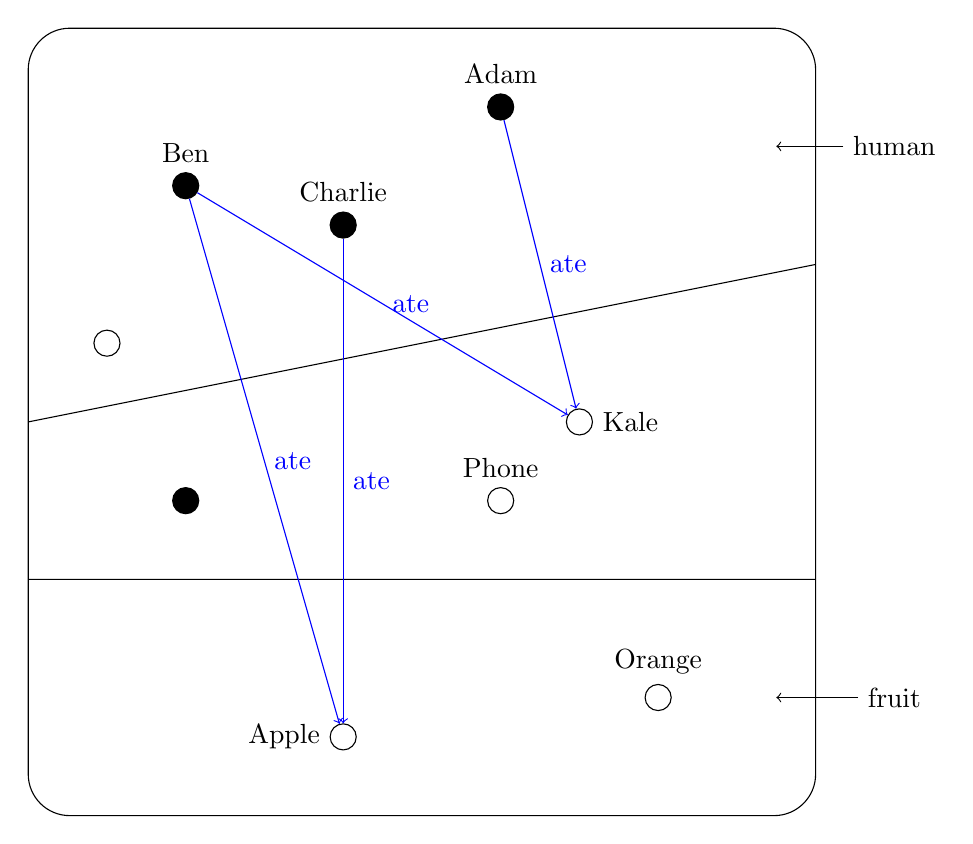
\begin{tikzpicture}
                \draw[rounded corners=15]
                (0, 0) -- (10, 0) -- (10, 10) -- (0, 10) -- cycle;

                \draw
                (0, 5) -- (10, 7)
                (0, 3) -- (10, 3);

                \node[] (human) at (11, 8.5) {human};
                \node[] (fruit) at (11, 1.5) {fruit};
                \draw
                (human) edge[->] node{} (9.5, 8.5)
                (fruit) edge[->] node{} (9.5, 1.5);

                \node[draw, circle, label=, fill=black] () at (2, 4) {};
                \node[draw, circle, label=Charlie, fill=black] (charlie) at (4, 7.5) {};
                \node[draw, circle, label=Adam, fill=black] (adam) at (6, 9) {};
                \node[draw, circle, label=Ben, fill=black] (ben) at (2, 8) {};
                \node[draw, circle, label=] () at (1, 6) {};
                \node[draw, circle, label=right:Kale] (kale) at (7, 5) {};
                \node[draw, circle, label=Phone] (phone) at (6, 4) {};
                \node[draw, circle, label=left:Apple] (apple) at (4, 1) {};
                \node[draw, circle, label=Orange] (orange) at (8, 1.5) {};

                \draw
                (ben) edge[->, right, color=blue] node{ate} (kale)
                (ben) edge[->, right, color=blue] node{ate} (apple)
                (adam) edge[->, right, color=blue] node{ate} (kale)
                (charlie) edge[->, right, color=blue] node{ate} (apple);
            \end{tikzpicture}
        \end{center}
        \textbf{NOTATION:} given an $L$-structure $M$, and a constant $c$ in $L$, we use the notation $c^M$ to denote the interpretation of $c$ in $M$. $c$ is an object in dom($M$) that $c$ names in $M$. Therefore the black node in the model, is $\texttt{Adam}^M$, which is not to be confused with \texttt{Adam}. The meaning of a constant $c$ is the object $c^M$, which is assigned by the $L$-structure $M$, hence a constant can have multiple meanings since each $L$-structure assigns $c$ a new meaning.
        \medskip

        While our model is quite simple, it illustrates the basic requirements for an $L$-structure; it has the collection of objects (dom($M$)), marks the constants, marks which objects satisfy the unary relations, as well as directed arrows showing which pairs of objects satisfy the binary relations. Generally, there isn't any easy way to represent $n$-ary relations (where $n \geq 3$). 0-ary (nullary) relations are propositional atoms.
        \medskip

        The structure $M$ tells us that \texttt{student}(\texttt{Ben}) is true, as the node representing $\texttt{Ben}^M$ is coloured black; therefore this can be written as $M \vDash \texttt{student}(\texttt{Ben})$ - or $M$ says \texttt{student}(\texttt{Ben}). $M$ also tells us that \texttt{ate}(\texttt{Ben}, \texttt{Orange}) is false, hence we can write $M \nvDash \texttt{ate}(\texttt{Ben},\ \texttt{Orange})$. $M$ also states $\texttt{Kale}^M$ is not \texttt{human}, therefore we are able to write $M \vDash \neg \texttt{human}(\texttt{Kale})$.
        \medskip

        This is a different use of $\vDash$ from the start of the module.
        \medskip

        \texttt{There should be a section here about another model on the same signature, but that \\ takes too much effort to draw.}
        \medskip

        \textbf{TIP:} if you have something asking $M \vDash \forall x (R(x, ...) \rightarrow B)$?, the idea is to restrict the $\forall x$. We know that falsity implies anything from propositional logic, and therefore we only need to consider the cases in which $R(x, ...)$ is true. For example, on $M$, if we were asked $M \vDash \forall x (\texttt{ate}(\texttt{Adam}, x) \rightarrow \texttt{ate}(\texttt{Ben}, x))$?, instead of evaluating all the objects in dom($M$), we should only consider the ones in which $\texttt{ate}(\texttt{Adam}, x)$ evaluates to true, which would be just the object $\texttt{Kale}^M$. And as $\texttt{ate}(\texttt{Ben}, \texttt{Kale}^M)$ is true, the statement is valid.
        \medskip

        \textbf{TIP:} for a fairly complex formula (we'll work with $\exists x (\texttt{fruit}(x) \land \exists y (\texttt{ate}(y, x)))$), a simple method is to work out what each subformula says in English (working upwards from the atomic subformulas). For example;
        \begin{center}
            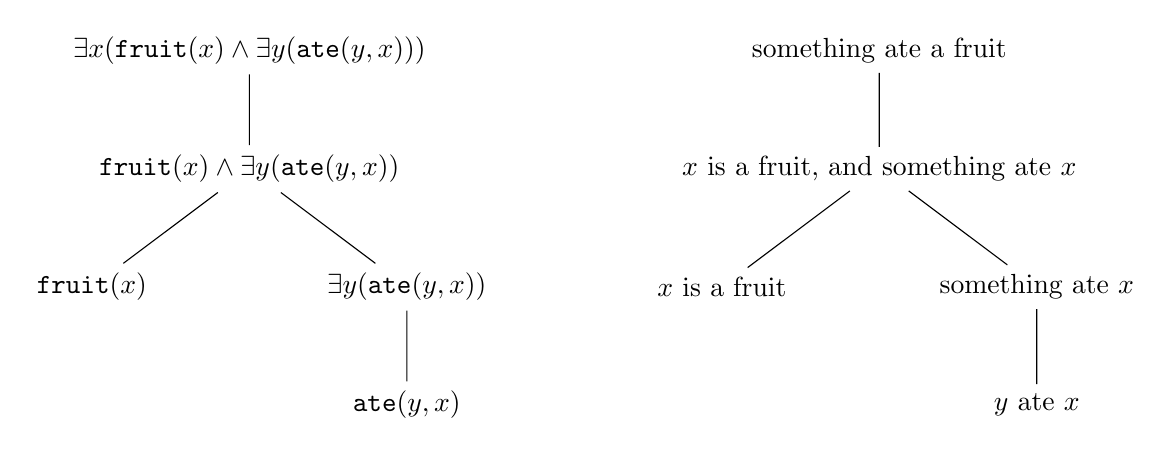
\begin{tikzpicture}
                \node[] (l_r) at (0, 0) {$\exists x (\texttt{fruit}(x) \land \exists y (\texttt{ate}(y, x)))$};
                \node[] (l_rc) at (0, -1.5) {$\texttt{fruit}(x) \land \exists y (\texttt{ate}(y, x))$};
                \node[] (l_rcl) at (-2, -3) {$\texttt{fruit}(x)$};
                \node[] (l_rcr) at (2, -3) {$\exists y (\texttt{ate}(y, x))$};
                \node[] (l_rcrc) at (2, -4.5) {$\texttt{ate}(y, x)$};

                \node[] (e_r) at (8, 0) {something ate a fruit};
                \node[] (e_rc) at (8, -1.5) {$x$ is a fruit, and something ate $x$};
                \node[] (e_rcl) at (6, -3) {$x$ is a fruit};
                \node[] (e_rcr) at (10, -3) {something ate $x$};
                \node[] (e_rcrc) at (10, -4.5) {$y$ ate $x$};

                \draw
                (l_r) -- (l_rc)
                (l_rc) -- (l_rcr)
                (l_rc) -- (l_rcl)
                (l_rcr) -- (l_rcrc)
                (e_r) -- (e_rc)
                (e_rc) -- (e_rcr)
                (e_rc) -- (e_rcl)
                (e_rcr) -- (e_rcrc);
            \end{tikzpicture}
        \end{center}
        \subsubsection*{Truth in a Structure (Formal)}
        Once again, natural language is only a rough guide, and as engineers we need a more rigorous system. While we are able to work out the truth value of a complex formula by evaluating propositional atoms from the root of a formation tree in propositional logic, it's not as simple in predicate logic. For example, if we tried to evaluate $\forall x (\texttt{ate}(\texttt{Charlie}, x) \rightarrow \texttt{fruit}(x))$ with a formation tree, we'd quickly run into trouble;
        \begin{center}
            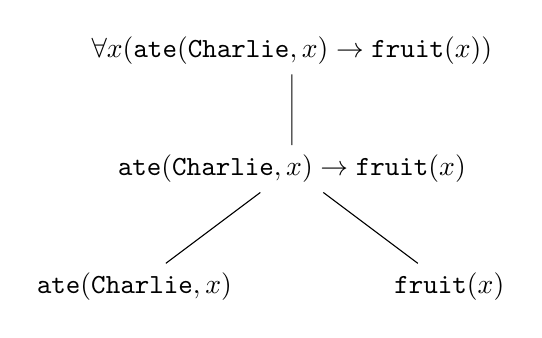
\begin{tikzpicture}
                \node[] (o) at (0, 0) {$\forall x(\texttt{ate}(\texttt{Charlie}, x) \rightarrow \texttt{fruit}(x))$};
                \node[] (oc) at (0, -1.5) {$\texttt{ate}(\texttt{Charlie}, x) \rightarrow \texttt{fruit}(x)$};
                \node[] (ocl) at (-2, -3) {$\texttt{ate}(\texttt{Charlie}, x)$};
                \node[] (ocr) at (2, -3) {$\texttt{fruit}(x)$};

                \draw
                (o) -- (oc)
                (oc) -- (ocl)
                (oc) -- (ocr);
            \end{tikzpicture}
        \end{center}
        What are the truth values for the leaf nodes? We don't know, since formulas of predicate logic doesn't have to be true or false in a given structure.
        \medskip

        With a given formula $A$, a variable $x$ in an atomic subformula of $A$ is \textbf{bound} if it's under a quantifiers in the formation tree. Otherwise, the variable is \textbf{free}. For example (copied directly from \textit{First-order logic.pdf});
        \begin{center}
            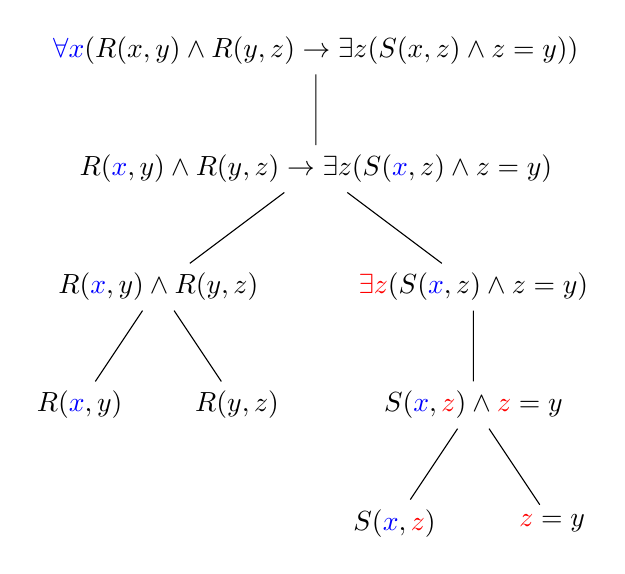
\begin{tikzpicture}
                \node[] (o) at (0, 0) {$\textcolor{blue}{\forall x} (R(x, y) \land R(y, z) \rightarrow \exists z (S(x, z) \land z = y))$};
                \node[] (oc) at (0, -1.5) {$R(\textcolor{blue}{x}, y) \land R(y, z) \rightarrow \exists z (S(\textcolor{blue}{x}, z) \land z = y)$};
                \node[] (ocl) at (-2, -3) {$R(\textcolor{blue}{x}, y) \land R(y, z)$};
                \node[] (ocr) at (2, -3) {$\textcolor{red}{\exists z} (S(\textcolor{blue}{x}, z) \land z = y)$};
                \node[] (ocll) at (-3, -4.5) {$R(\textcolor{blue}{x}, y)$};
                \node[] (oclr) at (-1, -4.5) {$R(y, z)$};
                \node[] (ocrc) at (2, -4.5) {$S(\textcolor{blue}{x}, \textcolor{red}{z}) \land \textcolor{red}{z} = y$};
                \node[] (ocrcl) at (1, -6) {$S(\textcolor{blue}{x}, \textcolor{red}{z})$};
                \node[] (ocrcr) at (3, -6) {$\textcolor{red}{z} = y$};

                \draw
                (o) -- (oc)
                (oc) -- (ocl)
                (oc) -- (ocr)
                (ocl) -- (ocll)
                (ocl) -- (oclr)
                (ocr) -- (ocrc)
                (ocrc) -- (ocrcl)
                (ocrc) -- (ocrcr);
            \end{tikzpicture}
        \end{center}
        The coloured variables are bound, and the uncoloured ones are free. Notice that $z$ occurs as both a free, and as an unbound variable. The two instances of $z$ are different, and have nothing to do with each other.
        \medskip

        A \textbf{sentence} is defined as a formula without any free variables (hence all variables are bound).
    \end{document}